Tout mon stage n'a pas été dédié uniquement à étudier des appareils caméras. J'ai également eu la charge d'établir un benchmark d'algorithmes de suivi fournis avec OpenCV.

\section{Benchmark d'algorithmes avec Open CV}

Durant mon stage, j'ai eu l'opportunité d'utiliser l'API \textbf{OpenCV} pour Python. Cette partie présente d'abord OpenCV, puis la mission qui m'a été confiée de réfléchir à des tests pour comparer des algorithmes de Computer Vision.
  \subsection{Présentation d'Opencv}
  
\begin{minipage}{0.2\textwidth}
  \centering
  
\includegraphics[width=2cm]{img/opencv.png}
\end{minipage}
\hfill%
\begin{minipage}{0.7\textwidth}

  \textit{OpenCV}~\cite{aboutOpenCV} (Open Source Computer Vision Library) est une librairie open source de \textit{Computer Vision} et de \textit{Machine Learning}. Avec une licence BSD, \textit{OpenCV} est simple à utiliser et à modifier pour les business.

\end{minipage}\par
  
La librairie comporte plus de 2500 algorithmes, allant des algorithmes classiques de \textit{Machine Learning} et de \textit{Computer Vision} aux plus modernes. Ces algorithmes permettent notamment de détecter et de reconnaître des objets, tracer les mouvements des objets, ou encore du traitement d'image.

\textit{OpenCV} a des interfaces \textit{C++, Python, Java} ainsi que \textit{MATLAB} et il supporte \textit{Windows, Linux, Android} et \textit{Mac OS}. \textit{OpenCV} continue d'étendre ses compatibilités. Par exemple, une interface pour être utilisé par les processeurs graphiques Nvidia utilisant \textit{ CUDA} est actuellement en cours de développement. La version d'\textit{OpenCV} utilisée durant ce stage est la version \textit{Python} 3.4.1.

  \subsection{Objectif: tests d'algorithmes de tracking}
  
  Cette mission consiste à établir des tests pour comparer différents algorithmes. Ceci passe par la détermination de critères à évaluer et de la mise en place d'une solution pour les évaluer.
  
  \subsubsection{État de l'art}

  \subTrois{Le tracking d'objet}
    
      Le tracking d'objet lui même est la tâche de suivre un ou plusieurs objets dans une scène, de la première apparition à la sortie. Un objet peut être n'importe quel objet qui peut être détecter dans une séquence d'image~\cite{trackingSotA1}. Il peut s'agir d'une voiture qui traverse une intersection. En général, dans un environnement dynamique l'objet et le fond sont susceptibles de changer. La voiture par exemple peut tourner et ainsi changer d'angle de vue et de taille avec la perspective. Le fond avec l'évolution de la luminosité au fil de la journée ou un mouvement de caméra.
  
  En principe la résolution de ces problèmes est complexe. Il est nécessaire de mettre en place une série de contraintes pour qu'il puisse devenir résoluble. Parmi les contraintes qui peuvent aider avec les problématiques de la Computer Vision on compte~:
\begin{itemize}[noitemsep]
  \item Une caméra fixe
  \item Un nombre d'objet connu
  \item La taille des objets connue
  \item Une obstruction des objets limitée
  \item Un déplacement des objets fluide
  \item Pas de changement brutal du fond ou des objets
\end{itemize}
  
    Une fois ces contraintes établies pour générer les vidéos qui serviront de base de travail, des \textit{API} avec leurs lots de solutions existent pour répondre aux besoins en \textit{Computer Vision}. On retiendra principalement celles d'\textbf{Opencv}, tout en s’intéresserant aussi à d'\textbf{autres solutions généralistes}.
    
        Dans la computer Vision, plusieurs types d'algorithmes sont utilisés. Des algorithmes de \textbf{détection}, de \textbf{reconnaissance} et \textbf{tracking}~\cite{Reco}.

    \subTrois{Les solutions fournies par OpenCV}
    \textit{OpenCV} est une librairie qui fournit des API de détection, de reconnaissance et de tracking.
    
        \subQuatre{API de détection}
        OpenCV permet d'utiliser des algorithmes pour détecter un objet sur une image. Un algorithme de détection permet de détecter automatiquement un objet. Cette reconnaissance peut se faire en se focalisant sur les objets en mouvement. Toutefois, cette méthode peut être confrontée à des limitations quand il s'agit d'observer un objet immobile ou obstrué par un objet au premier plan.

Sur OpenCV on retrouve une variété d'algorithmes via son API, dont \textbf{HAAR Cascade}~\cite{HaarOpenCV} qui repose sur du Machine Learning.

Cette méthode peut être utilisée pour suivre un objet image après image, mais risque de le perdre quand il se retrouve à l'arrêt.
      \subQuatre{API de reconnaissance}
        Une fois un objet détecté, il peut être utile de le reconnaître. Dans ce cas, il est nécessaire d'associer les points d’intérêts de l'objet (\textit{features}) à ceux d'une galerie d'objet que l'algorithme a été entraîné à reconnaître.
        
  Les objets que l'on a besoin de reconnaître sont très liés au contexte, les algorithmes de détection sont souvent spécialisés.  Par exemple, depuis Open CV 2.4, une API de reconnaissance de visage est inclue~\cite{FaceReco}.
      \subQuatre{API de tracking}
    Les algorithmes de tracking permettent de suivre un objet. l'algorithme va comparer l'évolution entre plusieurs images successives dans une vidéo. Ces algorithmes permettent de suivre un objet, qu'il se déplace ou non. À la différence d'un algorithme de détection, ils ne permettent pas de repérer automatiquement un objet si on ne le lui pas indiqué initialement. Certains algorithmes sont plus fluides que d'autres, gèrent mieux le changement d'angle de la prise de vue ou de tailles d'un objet, tiennent compte de la perte d'un objet qu'il est supposé suivre.
    
  OpenCV intègre dans sa version 3.4.1 plusieurs fonctions de tracking prête à l'emploi. La plus ancienne \textbf{BOOSTING} a une dizaine d'années alors que les plus récentes comme \textbf{CSRT} ont été ajoutées dans la version la plus récente de l'API.~\cite{APItracking}  
                
  \subTrois{Autres solutions généralistes existantes}
     
       De nombreuses solutions pour le tracking d'objets existent actuellement. Certaines de ces solutions sont apportées par des API de Computer Vision prêtes-à-l'emploi provenant de grands groupes comme \textit{Google}, \textit{Microsoft} et \textit{IBM}~\cite{trackingSotA2}. Cependant ces outils universels ne sont pas toujours utile. Une solution plus spécialisée à un problème donné peut être plus efficace pour sa résolution.
       

\begin{minipage}{0.3265\textwidth}
\begin{figure}[H]
  \centering
  
\includegraphics[width=3cm]{img/tensorflow.png}
    \caption{\\Google Tensorflow}
\end{figure}
\end{minipage}
\begin{minipage}{0.34\textwidth}
\begin{figure}[H]
  \centering
  
\includegraphics[width=3cm]{img/MicrosoftCS.png}
    \label{MS Cognitive Service}
    \caption{MS\\Cognitive Service}
\end{figure}
\end{minipage}
\begin{minipage}{0.3265\textwidth}
\begin{figure}[H]
  \centering
  
\includegraphics[width=3cm]{img/IBM_Watson_Logo_2017.png}
    \caption{\\Watson d'IBM}
\end{figure}
\end{minipage}

Aujourd'hui les algorithmes dans des compétitions de reconnaissance d'objet ne sont toujours pas capable d'avoir des résultats parfaits dans le tracking d'objets multiples~\cite{MOT16}.

  \subsubsection{Contribution sur OpenCV}
     \subTrois{Pertinence et difficulté} Ma mission concerne l'analyse des algorithmes de fonctions de \textbf{suivie} (ou \textbf{tracking}) d'OpenCV.
     
     En effet, les algorithmes concernés serviront à analyser le flux de la circulation routière et piétonne filmé par des caméras de sécurité. Les éléments à tester sont~:
     \begin{itemize}
\item La \textbf{reconnaissance} des objets en premier plan.
\item L’\textbf{identification} des objets en premier plan.
\item Le \textbf{parcours} des objets
\item La \textbf{vitesse d’exécution} en fonction du nombre d’objets et de la résolution de l’image.
\end{itemize}
  
    Les solutions retenues pour chacun de ces points doit tenir en compte des particularités de ce contexte. Parmi ces particularités on peut retenir que l'image est fixe, la qualité risque de varié en fonction de la météo, les zones piétonnes et routières ne varient pas, les objets en mouvement sont des véhicules de tout types et des piétons.
    
    \subTrois{Résolution}
    
    La résolution des difficultés passe par la mise en place matérielle et logicielle du test, et par l'étude des critères à analyser.
    
    \subQuatre{La mise en place}
  Ces tests pour avoir des résultats comparables devront être réalisés sur du matériel avec une configuration connue afin d'éviter les écarts de performance liés au matériel alors que l'on souhaite évaluer les performances du logiciel.
        
  Afin d'avoir des tests reproductibles et que les données attendues soient prévisibles, le flux vidéo qu'analyseront ces algorithmes de \textit{Computer Vision} sera constitué de vidéos enregistrés et correspondant à différentes situations (de circulation ou météorologiques par exemple) pour couvrir au maximum l'efficacité des algorithmes.

    En vue d'établir un benchmark qui répond au mieux aux besoins en l'espèce, deux angles ont été retenus, la précision de l'identification et la vitesse d'exécution.

    \subQuatre{La précision}
    L'algorithme a pour mission d'identifier et de cataloguer les objets filmés et leurs déplacements dans le cadre.

Ces résultats doivent être catalogués dans un log. On attend du log de contenir les objets en mouvement identifiés, les objets reconnus et leurs parcours au travers de différentes zones. Ce log sera analysé et comparé au résultat attendu.

Dans le cadre de la \textbf{reconnaissance} d'un objet en mouvement on peut rencontrer plusieurs cas. Un vrai positif, un objet à détecter a été détecté. Un faux négatif, un objet à détecter n'a pas été détecté. Un faux positif, un objet a été détecté alors qu'il n'y avait pas d'objet à détecter. L'analyse du log doit en tenir compte afin de ne pas favoriser un algorithme trop sensible qui détectera des objets là où rien n'est à analyser.

Pour l'\textbf{identification} d'un objet, soit un objet est correctement identifié soit il ne l'est pas. La situation est la même pour le \textbf{traçage de parcours des objets}. Ce traçage se fait en enregistrant l'entrée et la sortie dans des zones définies pour la caméra (trottoir, passage piété, voie à sens unique...).

L'analyse du log se conclut par l'établissement d'un score qui augmente en fonction des résultats identifiés comme vrai positif  et diminue en fonction des autres.

      \subQuatre{La vitesse d’exécution}
    Les algorithmes n'ont pas nécessairement la même vitesse d'exécution et plus elle est réduite, plus l'algorithme sera apte à analyser un flux continu.
    
    Le test tiendra simplement en compte la durée d'exécution et établira un score en fonction de la durée de la vidéo comme référence.
      \subQuatre{Implémentation}
\textbf{Sélections d'algorithmes de tracking~:}
        
Pour tester différents algorithmes de tracking rapidement,  une fenêtre de sélection de l'algorithme souhaité a été créée. Cette interface est faite en utilisant le module \textbf{tkinter} de \textit{Python}. Dans la liste des algorithmes se trouve pour l'instant les algorithmes inclus dans \textbf{OpenCV}. Ceci évite de modifier manuellement le code à chaque fois que je désire tester un algorithme différent.

% ------------------------------

On va s’intéresser à la partie qui consiste à la sélection d’un algorithme en passant par une interface graphique créée avec tkinker.

\begin{figure}[H]
  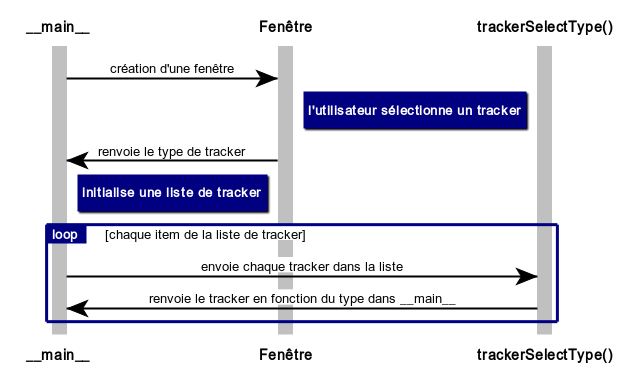
\includegraphics[width=14cm]{img/diag_seq.png}
    \centering
    \caption{Sélection et initialisation\\ de l'algorithme de tracking}
\end{figure}
La première étape est de créer une liste avec le nom de chaque algorithme.

  \begin{minted}[linenos, breaklines, frame=lines, label=Mise en place d'openCV sur Python et de la liste des algorithmes]{python}
import numpy as np
import cv2 as cv
import tkinter as tk
from tkinter.messagebox import showinfo

# Les différents types de trackers inclus dans l'API
    tracker_types = ['BOOSTING', 'MIL', 'KCF', 'TLD', 'MEDIANFLOW', 'GOTURN', 'MOSSE', 'CSRT']
\end{minted}

% ------------------------------
Cette liste va servir à créer une fenêtre avec une liste avec un item à sélectionner

\begin{minted}[linenos, breaklines, frame=lines, label=Fenêtre de sélection de l'algorithme]{python}
fenetre = tk.Tk()
liste = tk.Listbox(fenetre)
for track in tracker_types:
    liste.insert(tracker_types.index(track), track)
liste.pack()
bouton = tk.Button(fenetre,
          text = "Select",
          command = fenetre.quit)
bouton.pack()
fenetre.mainloop()

# Algorithme choisi
tracker_type = tracker_types[liste.curselection()[0]]
\end{minted}
\begin{figure}[H]
  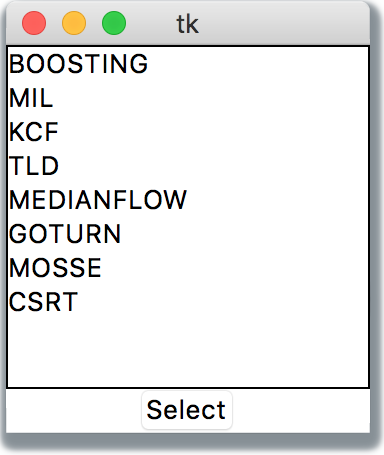
\includegraphics[width=3cm]{img/trackerbox.png}
    \centering
    \caption{boite de dialogue\\pour choisir le tracker}
\end{figure}

% ------------------------------
  On initialise une liste de trackers. Cette liste aura la taille du nombre de \textit{Bounding Box} créées. L'algorithme boosting est sélectionné par défaut afin de créer une liste de trackers, il va être écrasé par un autre tracker.
\begin{minted}[linenos, breaklines, frame=lines, label=Initialisation s'adaptant au nombre de bounding box]{python}
    bbox = [(290, 205, 40, 90),
            (605, 230, 40, 90),
            (700, 250, 40, 90)]
            
for i in range (0,len(bbox)):
        if i == 0:
            trackerselect = [cv.TrackerBoosting_create()]
        else:
            trackerselect.append(cv.TrackerBoosting_create())
    for i in range(0,len(bbox)):
        trackerselect[i] = trackerSelectType(trackerselect[i])
\end{minted}

% ------------------------------

  L'item sélectionné va servir à choisir la fonction pour initialiser un nouveau tracker qui va être inclus dans la liste des trackers. Il écrase le tracker par défaut. Il est nécessaire de repasser par cette fonction à chaque initialisation, autrement la liste de trackers pointera toujours vers le même tracker.

\begin{minted}[linenos, breaklines, frame=lines, label=Attribution de l'algorithme à des trackers]{python}
def trackerSelectType(trackerselect):
    (major_ver, minor_ver, subminor_ver) = (cv.__version__).split('.')
    if int(minor_ver) < 3:
            trackerselect = cv.Tracker_create(tracker_type)
    else:
        if tracker_type == 'BOOSTING':
            trackerselect = cv.TrackerBoosting_create()
        if tracker_type == 'MIL':
...
    return trackerselect
\end{minted}

% ------------------------------

\textbf{La vidéo et les régions d'intérêts des objets à suivre}

Comme on souhaite tester le tracking, les algorithmes sont utilisés dans des situations similaires. Pour cela le programme assure que l'on aura à chaque fois~:
\begin{itemize}[noitemsep]
\item La même vidéo.
\item Les mêmes zones d’intérêt sélectionnées. 
\end{itemize}
De légères différences dans la zone sélectionnée pour encadrer l'objet à suivre peuvent changer sensiblement le comportement de l'algorithme. Idéalement cette zone doit contenir au maximum l'objet avec un minimum d'arrière plan. Ceci peut être compliqué quand on analyse des formes non rectangulaires comme un cycliste sur son vélo.

Plusieurs vidéos ont été sélectionnées pour ce test. Une première, \textit{Shibuya} a été choisie car elle permet de voir la différence de comportement sur des objets de différentes tailles (voiture, bus, et arrière d'une voiture) et des obstacles (vue obstruée par le feu tricolore, la foule de piéton).

Les régions d'intérêts sont entrées dans un \textbf{tableau de tuples} (collection ordonnée d'attributs relatifs à un même objet) qui contiennent les coordonnées de chaque \textit{bounding box} (sélection rectangulaire de l'objet à suivre). L'utilisation de la bounding box se fait sous forme de boucle dont l'index s'adapte à la taille de se tableau de tuples. Ainsi en ajoutant ou retirant simplement un tuple dans ce tableau, le programme va pouvoir les suivre sans autre modification.

On peut déjà s'apercevoir en observant la vidéo que le comportement de ces \textit{Bounding Box} varie en fonction des algorithmes.

\begin{figure}[H]
  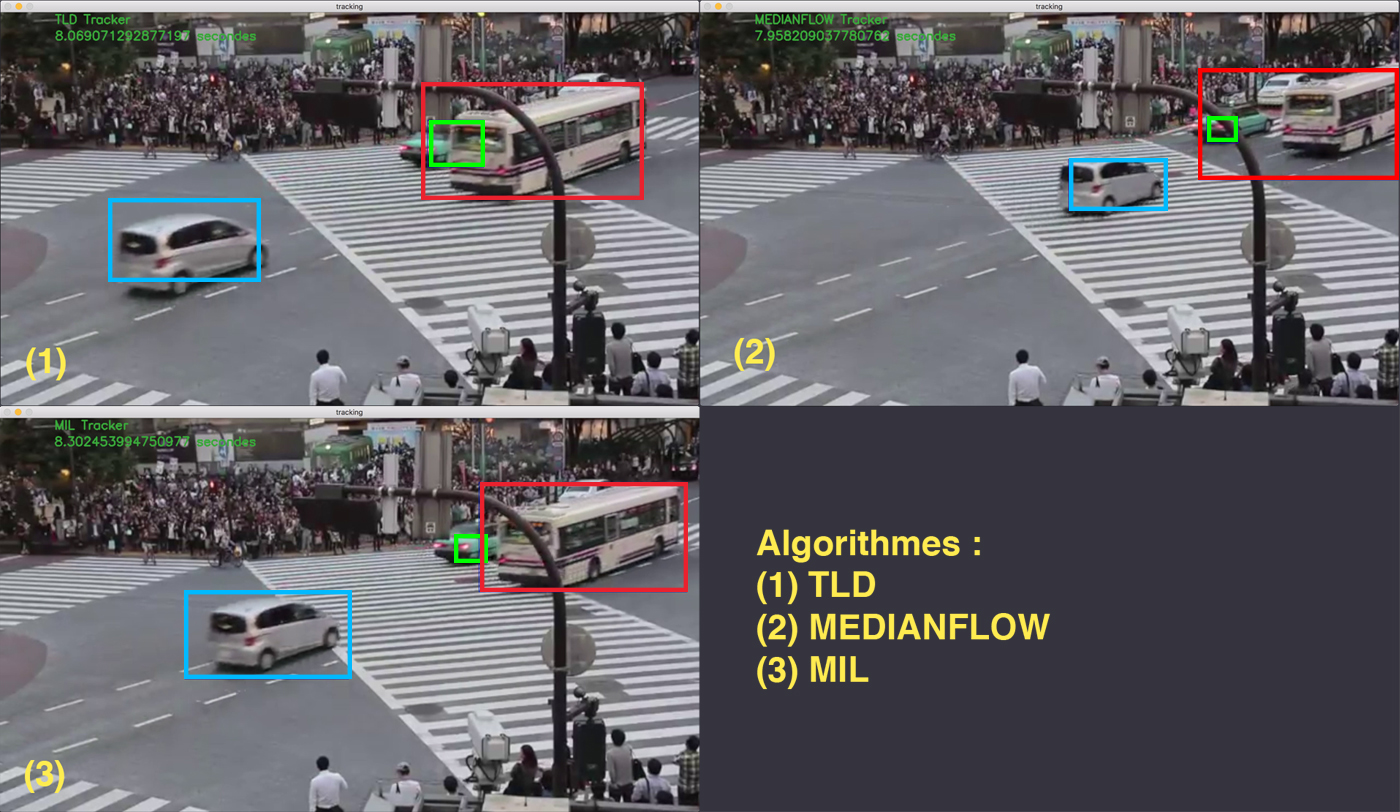
\includegraphics[width=0.7\textwidth]{img/algodiff.jpg}
    \centering
    \caption{Différence de résultats entre différents algorithmes à environ 8 secondes d'exécution.}
\end{figure}

Ces \textit{Bounding Box} vont avoir des temps d’exécutions plus ou moins long et vont parfois échouer à suivre chaque voiture sur la totalité de leur trajet. Avec ces informations, on peut commencer à l'élaborer un score pour chaque algorithme. L'incapacité à suivre des objets se déplaçant en ligne droite est éliminatoire et est indexé sur le temps d’exécution.

\begin{table}[H]
  \centering
  \label{my-label}
\begin{tabular}{|l|l|l|l|}
\hline
\rowcolor[HTML]{FFFFC7} 
Algorithme & Temps (secondes)   & Perte & \begin{tabular}[c]{@{}l@{}}Score\\ \tiny{\((3-Pertes) * (100/3)\)}\\\tiny{\( * ( Temps * Dur\acute{e}e)\)}\end{tabular}\\ \hline
Boosting   & 51.208574295043945 & 2     & 3,254663286                                                                     \\ \hline
MIL        & 54.95484709739685  & 2     & 3,032792838                                                                     \\ \hline
KCF        & 35.16063404083252  & 2     & 4,740149636                                                                     \\ \hline
TLD        & 110.28673601150513 & 3     & 0                                                                               \\ \hline
\textbf{MEDIANFLOW} & \textbf{24.363162994384766} & \textbf{0} & \textbf{20,5227868}                                                             \\ \hline
\end{tabular}
  \caption{Exemple de score pour différents algorithmes sur \textit{Shibuya}}
\end{table}

On peut alors observer sur cinq algorithmes un écart très important dans les temps d’exécution et la capacité à suivre un objet.

La vidéo \textit{Shibuya} a comme inconvénient un encodage qui conduit à une exécution très lente des algorithmes. La vidéo de \textbf{4,6 secondes} peut avoir un temps d’exécution de  l'algorithme TLD proche de \textbf{2 minutes}. Si cela peut être pénible lorsque l'on souhaite effectuer plusieurs tests successifs, ceci permet toutefois de mettre en exergue les différences de performances.

Lors de la suite de l'élaboration des tests, d'autres vidéos ont été privilégiées.

\textbf{Zones d'entrées et de sorties}

Un autre vidéo présente dans une intersection prise en coopération avec la ville cliente a servi pour les tests. Avec cette vidéo les temps d’exécution des algorithmes était bien plus proche de la durée de la vidéo.

Pour utiliser ces zones il a fallu choisir le critère pour déterminer quand un objet est ou non dans une zone. Pour cela les coordonnées Bounding Box sont exploitées. Plutôt que de considérer un objet comme dans une zone quand elle se superpose à la \textit{Bounding Box}, l'objet est considéré dans la zone quand son centre est dans la zone. 

Une fois ce critère choisi il a été possible d'afficher le parcours qu'effectue la \textit{Bounding Box} pour simplifier l'observation humaine. Dans ce même soucis d’observation, un message est affiché quand un objet est dans une zone. 

\begin{figure}[H]
  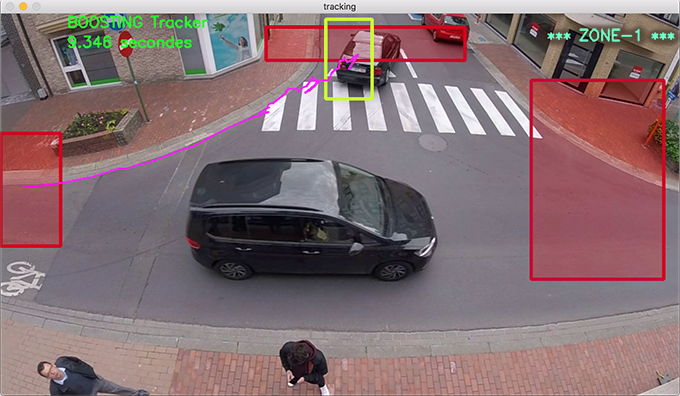
\includegraphics[width=0.6\textwidth]{img/ALGOZONE.png}
    \centering
    \caption{Objet entrant dans une zone}
\end{figure}

Il arrive que l'objet n'arrive pas à entièrement entrer dans la zone mais se superpose, choisir l'ensemble de la surface de la \textbf{Bounding Box} est plus favorable à produire des \textbf{faux positifs}.

\begin{figure}[H]
  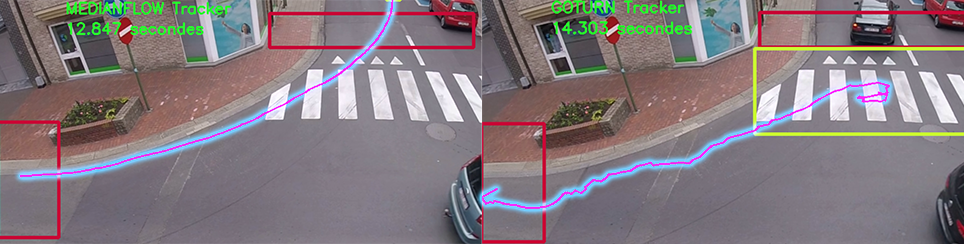
\includegraphics[width=0.9\textwidth]{img/path.png}
    \centering
    \caption{Différence de trajet entre deux algorithmes en magenta surligné}
\end{figure}

Dans le cas de figure de l'algorithme \textbf{Goturn}, l'objet était partiellement superposé dans la zone centrale. Choisir un paramètre plus restreint comme le centre a permis d'éviter un \textbf{faux positif}. 

\textbf{Création d'un log}

 Pour la création du log j'ai utilisé la librairie Python \textbf{logging}~\cite{log}. Cette librairie permet de simplement créer un fichier de log en fonction de l'activité du programme. Ce fichier a vocation à garder une trace de la dite activité et ainsi être utilisé pour comparer des résultats. Il enregistre quel algorithme est utilisé lors de la session, la position toute les trente frames, et quand l'objet entre et sort d'une zone.

\textbf{Élaboration d'un benchmark}

 % -------------------------`
 % -------------------------
 % |   |   |   |   |   |   |
 % -------------------------
  Pour affiner le benchmark par rapport au tableau de score précédent, des critères ont été ajoutés. Ces critères sont surtout qualitatifs et sont alors difficilement quantifiables. Avec la constatation des différences de performances entre les algorithmes, j'ai passé la vitesse d’exécution comme une variable qualitative. Au vu de la variabilité d'un critère comme les pertes en fonction de la vidéo, j'ai préféré en faire une variable qualitative en fonction de la capacité à ne pas perdre et sous le nom de «~\textit{Précision}~». 
% Please add the following required packages to your document preamble:
% \usepackage[table,xcdraw]{xcolor}
% If you use beamer only pass "xcolor=table" option, i.e. \documentclass[xcolor=table]{beamer}
\begin{table}[H]
\centering
\begin{tabular}{|c|c|c|c|c|c|}
\hline
\rowcolor[HTML]{3166FF} 
{\color[HTML]{FFFFFF} \textbf{Nom}}          & {\color[HTML]{FFFFFF} \textbf{Vitesse}}                         & {\color[HTML]{FFFFFF} \textbf{Adapte taille}}               & {\color[HTML]{FFFFFF} \textbf{\begin{tabular}[c]{@{}c@{}}repère\\ quand perdu\end{tabular}}} & {\color[HTML]{FFFFFF} \textbf{Fluidité}} & {\color[HTML]{FFFFFF} \textbf{Précision}} \\ \hline
\rowcolor[HTML]{F8A102} 
\cellcolor[HTML]{DAE8FC}\textbf{Boosting}    & {\color[HTML]{333333} \textbf{lent --}}                         & \cellcolor[HTML]{FE0000}{\color[HTML]{FFFFFF} \textbf{non}} & \cellcolor[HTML]{FE0000}{\color[HTML]{FFFFFF} \textbf{non}}                                  & \textbf{--}                              & \textbf{--}                               \\ \hline
\rowcolor[HTML]{FFFE65} 
\cellcolor[HTML]{DAE8FC}\textbf{MIL}         & {\color[HTML]{333333} \textbf{len -}}                           & \cellcolor[HTML]{FE0000}{\color[HTML]{FFFFFF} \textbf{non}} & \cellcolor[HTML]{FE0000}{\color[HTML]{FFFFFF} \textbf{non}}                                  & \textbf{-}                               & \textbf{-}                                \\ \hline
\cellcolor[HTML]{DAE8FC}\textbf{KCF}         & \cellcolor[HTML]{FFFE65}\textbf{lent -}                         & \cellcolor[HTML]{FE0000}{\color[HTML]{FFFFFF} \textbf{non}} & \cellcolor[HTML]{32CB00}\textbf{oui}                                                         & \cellcolor[HTML]{32CB00}\textbf{+}       & \cellcolor[HTML]{FFFE65}\textbf{-}        \\ \hline
\rowcolor[HTML]{FE0000} 
\cellcolor[HTML]{DAE8FC}\textbf{TLD}         & {\color[HTML]{FFFFFF} \textbf{lent ---}}                        & \cellcolor[HTML]{32CB00}\textbf{oui}                        & {\color[HTML]{FFFFFF} \textbf{non}}                                                          & {\color[HTML]{FFFFFF} \textbf{---}}      & {\color[HTML]{FFFFFF} \textbf{---}}       \\ \hline
\rowcolor[HTML]{32CB00} 
\cellcolor[HTML]{DAE8FC}\textbf{Median Flow} & \cellcolor[HTML]{FFFE65}\textbf{lent -}                         & \textbf{oui}                                                & \textbf{oui}                                                                                 & \textbf{+}                               & \textbf{+}                                \\ \hline
\cellcolor[HTML]{DAE8FC}\textbf{Goturn}      & \cellcolor[HTML]{F8A102}{\color[HTML]{333333} \textbf{lent --}} & \cellcolor[HTML]{32CB00}\textbf{oui}                        & \cellcolor[HTML]{FE0000}{\color[HTML]{FFFFFF} \textbf{non}}                                  & \cellcolor[HTML]{FFFE65}\textbf{-}       & \cellcolor[HTML]{F8A102}\textbf{--}       \\ \hline
\rowcolor[HTML]{32CB00} 
\cellcolor[HTML]{DAE8FC}\textbf{MOSSE}       & \cellcolor[HTML]{FFFE65}\textbf{lent -}                         & \cellcolor[HTML]{FE0000}{\color[HTML]{FFFFFF} \textbf{non}} & \textbf{oui}                                                                                 & \textbf{+}                               & \textbf{+}                                \\ \hline
\cellcolor[HTML]{DAE8FC}\textbf{CSRT}        & \cellcolor[HTML]{F8A102}\textbf{lent --}                        & \cellcolor[HTML]{32CB00}{\color[HTML]{333333} \textbf{oui}} & \cellcolor[HTML]{FE0000}{\color[HTML]{FFFFFF} \textbf{non}}                                  & \cellcolor[HTML]{32CB00}\textbf{+}       & \cellcolor[HTML]{FFFE65}\textbf{-}        \\ \hline
\end{tabular}
\caption{benchmark de différents algorithmes de tracking}
\end{table}



Un score n'est plus déduit, mais les différences restent facilement visibles.


  \subsection{Résultats et améliorations possibles}
    En l'état, le programme connaît encore plusieurs lacunes. 
    
    Il est fait pour lancer les algorithmes fournis par OpenCV. Cece le rend \textbf{limité par ces algorithmes implémentés de base}. Les algorithmes développés à part ne seront pas compatibles et demanderont des refontes importantes du programme pour y être utilisable. 
    
    Configurer le programme peut s'avérer \textbf{laborieux}. Sélectionner les zones d’intérêt se fait en rentrant des \textbf{coordonnées} d’abscisse, d'ordonnée, de longueur et de la largeur à la main.
Pour entrer un \textbf{temps} à laquelle une voiture est attendu dans une zone, il faut choisir une frame. Le temps en utilisant une horloge ne fonctionne pas car les algorithmes ont des temps d'exécutions différents. Trouver ces informations demande de procéder par tâtonnements et peut demander un nombre important d'essais.
    
    Également le programme n'est doté que d'une \textbf{faible automatisation}. Il n'est pas possible avec de programme d'automatiser avec certitude quand un objet entre ou sort d'une zone, car aucun de ces algorithmes de tracking n'est parfaitement fiable. 

  Parmi les objectifs posés lors de la réflexion autour des tests d'algorithmes de tracking se trouvaient les notions de \textbf{faux et vrais positifs}. Lors de la conception du programme je me suis retrouvé confronté à des problèmes pour reconnaître un faux positif. Par exemple, certains algorithmes ne sont pas capables de comprendre quand l'objet est perdu. Certains algorithmes peuvent voir leur zone d'analyse faire des «~sauts~» quand ils perdent l'objet et se retrouver dans la zone attendue. De même algorithme peut se mettre à suivre un mauvais objet quand il en croise un autre. 

 Effectuer un \textbf{benchmark} des algorithmes n'est pas parfaitement rigoureux. Les différences de vitesses changent en fonction de l'encodage de la vidéo. La capacité d'un algorithme à suivre un objet dépend grandement de la zone d’intérêt sélectionnée au départ. Il est possible qu'une zone d’intérêt favorise plus un algorithme qu'un autre.
 
 L'observation humaine reste essentielle dans ces tests.